\section{System Design}

% Authors: Keerthi Rapolu & Sreeja Katta

PBCP follows a Prevent -> Correct -> Learn pipeline. The system first infers what
the workload is trying to do, estimates whether the request is likely to waste
compute, and applies a pre-billing intervention when the expected savings justify
the action. Once a workload is running, PBCP continues to monitor for divergence
between declared intent and observed behavior, applies runtime corrections when
needed, and feeds those outcomes back into future governance decisions.

\subsection{Overview}

Figure~\ref{fig:architecture} illustrates the full
Prevent~$\rightarrow$~Correct~$\rightarrow$~Learn pipeline. A workload enters
the system as a natural-language submission, is converted into a structured
workload-intent representation, is compared with historical analogs, and is then
evaluated by a pre-execution simulator and expected-value decision engine before
resources are launched.

\begin{figure}[t]
\centering
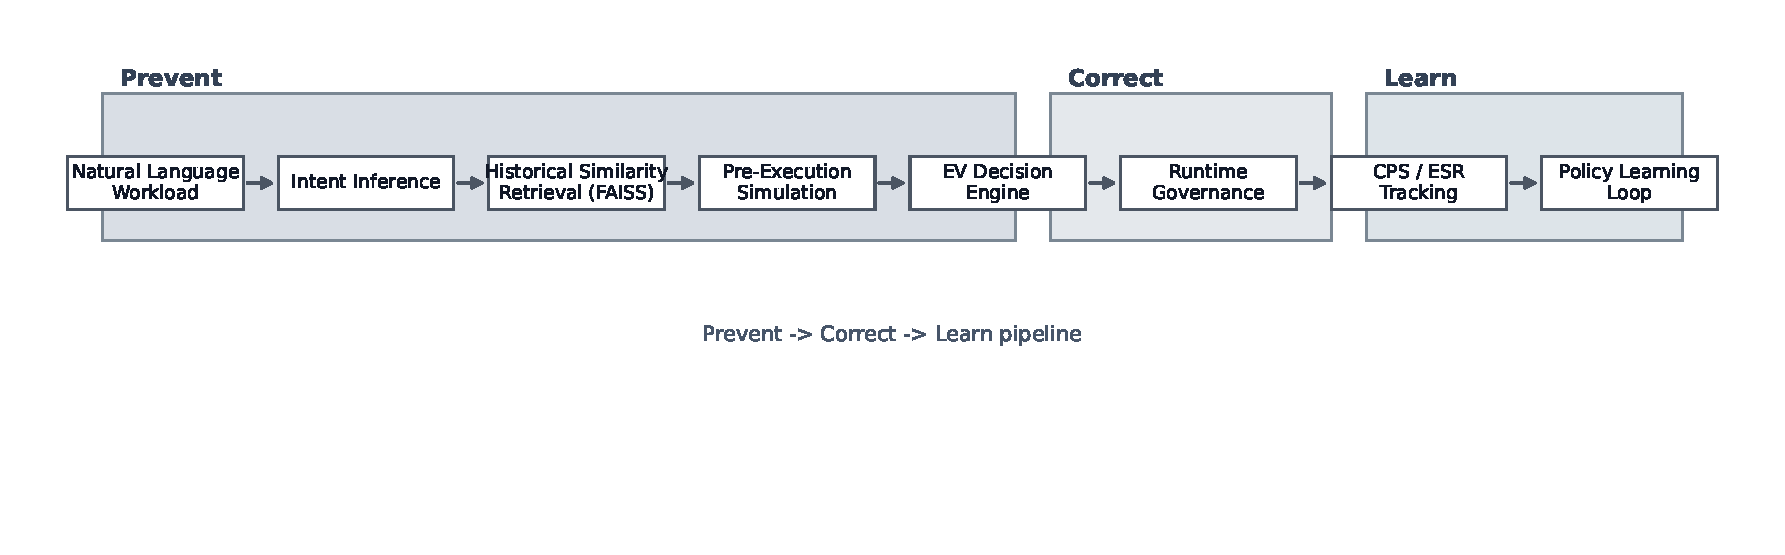
\includegraphics[width=\linewidth]{figures/architecture_overview.pdf}
\caption{PBCP system architecture. The pipeline groups pre-billing prevention, runtime correction, and policy learning into one governance loop.}
\label{fig:architecture}
\end{figure}

The figure also shows why PBCP is not only a pre-provision filter. Prevention,
runtime governance, and policy learning operate as a continuous control loop so
that early intervention, online correction, and later policy adaptation all
share the same workload-alignment view.

\subsection{Intent Inference}

Intent inference converts the submitted description, request metadata, and
available team history into a structured workload-intent representation. This
representation captures workload type, recurrence, urgency, sensitivity, and
resource expectations before execution begins. The purpose is operational rather
than descriptive: governance needs an early estimate of what the workload is
trying to do so that later decisions are conditioned on expected behavior rather
than on telemetry alone.

\subsection{Historical Similarity Retrieval}

Historical similarity retrieval uses FAISS to query prior workload-intent
representations and recover nearby examples with similar execution profiles.
These neighbors provide empirical priors for likely utilization, duration, and
waste patterns. In effect, retrieval grounds governance in observed workload
history rather than relying only on static workload classes. When close matches
are unavailable, PBCP falls back to catalog-level priors so that the system
remains usable under cold-start conditions.

\subsection{Pre-Execution Simulation}

The pre-execution simulator combines workload intent with historical priors to
estimate likely utilization, duration, cost, and right-sized capacity if the
request is executed unchanged. This stage turns workload intent into a concrete
governance forecast. Instead of waiting for a job to become visibly inefficient,
PBCP estimates whether the requested configuration is already likely to diverge
from expected behavior before provisioning occurs.

\subsection{EV Decision Engine}

The expected-value decision engine compares the outcomes of
\texttt{BLOCK}, \texttt{AUTO\_CORRECT}, \texttt{SUGGEST}, and \texttt{PASS} by
balancing predicted prevented cost against intervention cost, delay, and failure
risk. This decision-theoretic step matters because governance is not free:
aggressive intervention can reduce waste while also increasing execution risk.
PBCP therefore treats pre-billing intervention as a cost-sensitive control
problem rather than as a fixed rule trigger.

\subsection{Runtime Governance}

Runtime governance monitors launched workloads for divergence patterns that are
not fully observable before execution, including prolonged idle periods,
underutilized clusters, and runaway execution. It serves as a second line of
defense rather than a replacement for pre-billing intervention. This distinction
is important for governance timing: even an accurate simulator cannot eliminate
all uncertainty, so runtime correction remains necessary when workload alignment
breaks down only after launch.

\subsection{Intent-Behavior Discrepancy (IBD)}

This stage introduces intent-behavior divergence as the mismatch between
declared workload intent and observed runtime behavior. IFS provides the
corresponding workload-alignment signal by measuring semantic alignment between
intent and behavior. Within PBCP, this signal supports both anomaly diagnosis
and later policy learning, making it possible to distinguish low utilization
that is expected from low utilization that indicates governance failure.

% Authors: Keerthi Rapolu & Sreeja Katta

IFS maps the embedding cosine to four alignment categories: \emph{well-aligned}
($\mathrm{IFS} \geq 0.85$), \emph{minor divergence} ($0.70 \leq \mathrm{IFS}
< 0.85$), \emph{significant divergence} ($0.50 \leq \mathrm{IFS} < 0.70$), and
\emph{severe divergence} ($\mathrm{IFS} < 0.50$). These thresholds are chosen
so that the IBD flag ($\mathrm{IFS} < 0.65$) falls between the minor and
significant bands, giving anomaly detection a conservative operating point that
does not require separate threshold calibration.

The score decomposes into four interpretable sub-scores — type alignment,
utilization alignment, duration alignment, and resource alignment — weighted
0.35, 0.25, 0.20, and 0.20 respectively. For LLM pipeline workloads, a
token-waste sub-score replaces part of the resource term because token budget
adherence carries governance significance that node count alone does not capture.
These sub-scores are presented in the dashboard as interpretability support
rather than as standalone metrics; the canonical IFS value remains the embedding
cosine.

The role of IFS within PBCP is diagnostic rather than preventive. A workload can
receive high CPS because an effective intervention was applied and high IFS
because runtime behavior remained aligned, or low CPS because no intervention
was triggered and low IFS because the job behaved contrary to its stated intent.
That separation is what makes IFS useful: it explains why waste occurred rather
than only measuring whether it was stopped, and it gives the policy learning loop
a signal that CPS and ESR do not directly capture.


\subsection{Policy Learning Loop}

The policy-learning loop closes the system by feeding repeated divergence
patterns, missed savings opportunities, and successful interventions back into
future governance decisions. Over time, this allows PBCP to move beyond a fixed
set of preconfigured rules and improve intervention quality through accumulated
workload evidence. In this sense, policy learning is not a separate analytics
feature; it is the mechanism that allows governance timing to improve across
successive workload generations.
